\chapter{High Frequency Trading}

High frequency trading (HFT) strategies are based on buy and sell assets in
short periods of time gaining a small profit in every transaction, the key is
the amount of transactions that algorithms are capable to execute obtaining profit considering transaction costs. 
In 2012 more than 50\% of US market share of exchange trades were HFT.  HFT has
motivated computer-driven strategies capable of processing large amount of data
in short periods of time. 


\section{High Frequency Trading}

HFT is not a strategy but a technology which allow to implement particular
trading strategies. The aim of HFT is to benefit from market short-term pricing
inefficiencies~\cite{chlistalla2011}. HFT is characterised for the use of
high-speed and sophisticated quantitative and algorithmic computer applications
for modelling and executing orders efficiently. In order to make fast decisions,
HFT firms require speed access to trading center servers and sometimes they are
physically near minimising network latencies.

High frequency trades are short-term positions that commonly end the trading
day avoiding leaving opened positions to the next business day. HFT is
frequently associate to algorithm trading strategies, but the former is focused
in to reduce the market impact of large institutional positions and the later refers to trade execution strategies that are typically used by fund managers to buy or sell large amounts of assets. The duration of the positions in HFT it is not well-defined. Figure~\ref{fig:HFTtimes} shows a survey done to traders about the holding time
of a position opened. Most of them agreed that HFT refers to positions between
1-second and 10-minutes. Overnight positions are avoided since they are more
risky and also have more expensive fees, HFT firms end the trading day closing all
opened positions.

\begin{figure}[!h]
  %\vspace{-0.8cm}
  \centering
  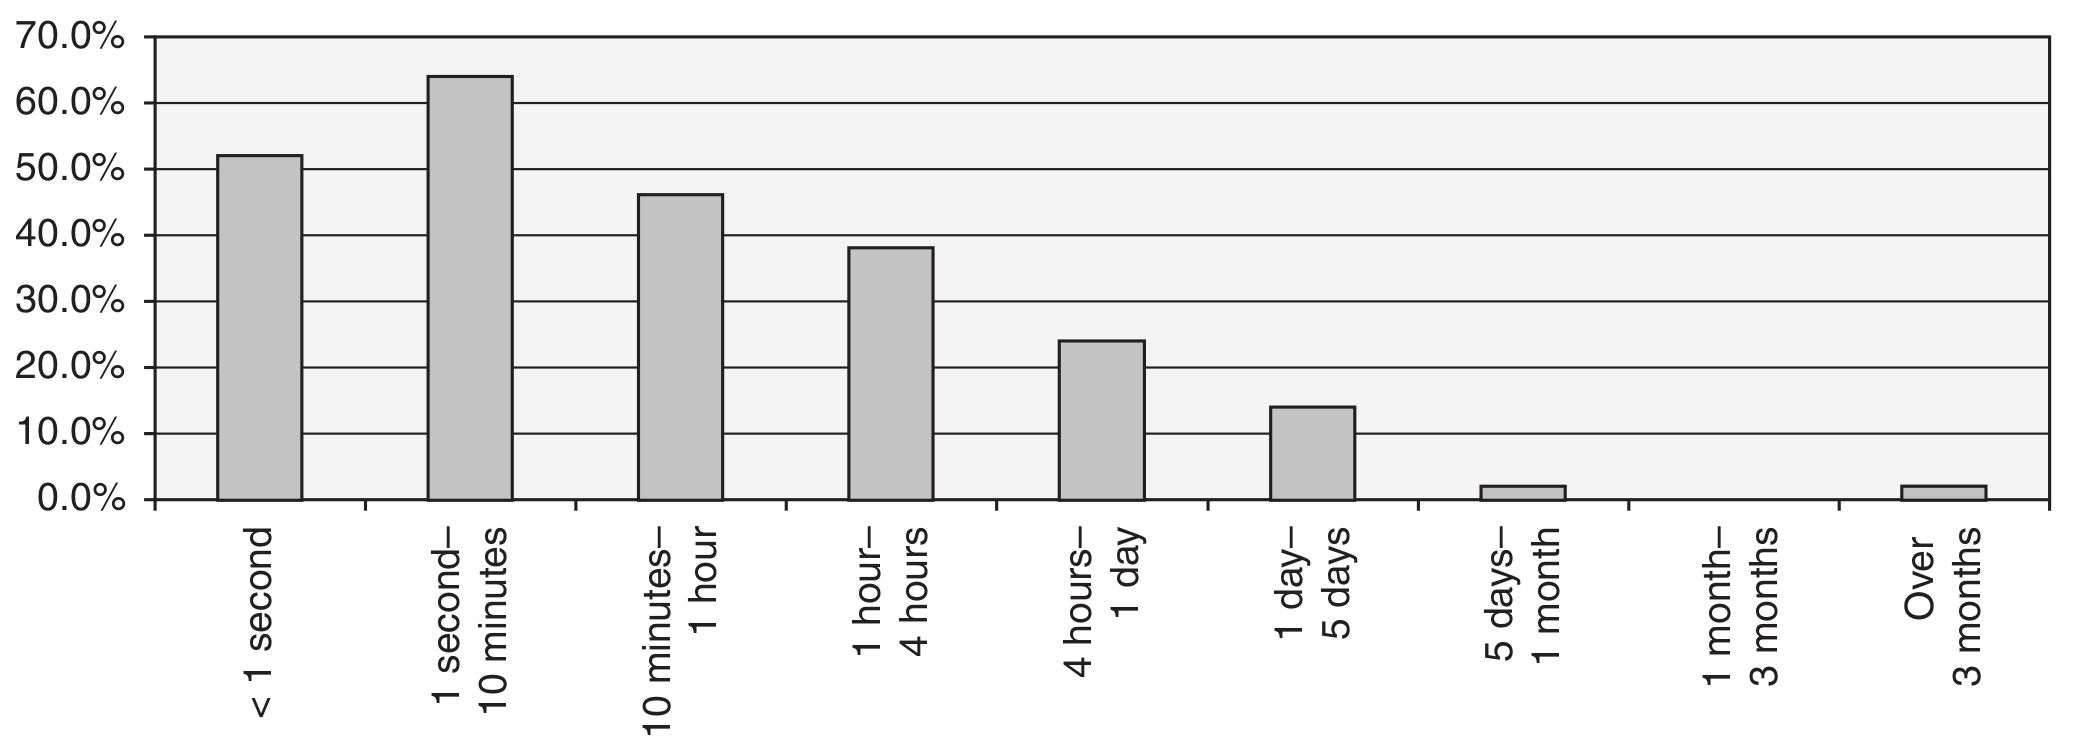
\includegraphics[width=\textwidth]{img/HFTtradestime}
  \caption{Holding time of an opened position of a high frequency trade.}
  \label{fig:HFTtimes}
\end{figure}
In 2014 HFT represented nearly 50\% of equity trades in the US and more than 20\%
in Europe showing a consistent fall since 2009 which was its best year. US market Revenues
have fallen dramatically.
Figure~\ref{fig:HFTmarket} on the left shows HFT trades percentage of US and Europe equity shares. The right figure shows how revenues in US stocks have fallen the last years.

\begin{figure}[!h]
  %\vspace{-0.8cm}
  \centering
  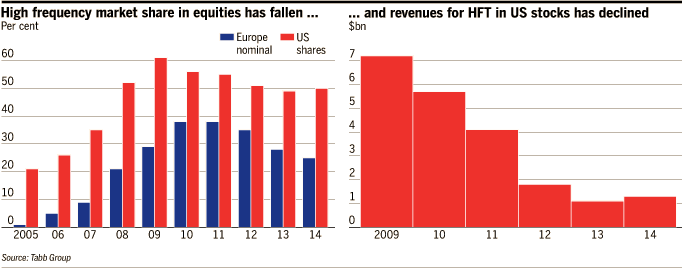
\includegraphics[width=\textwidth]{img/HFTmarket}
  \caption{Left figure shows HFT market share in the US and Europe. Right figure
  shows revenue in the US.}
  \label{fig:HFTmarket}
\end{figure}
One of the reasons of this fall is that exchange markets have adapted, having
now faster and more transparent and efficient market structures than before.
This has been possible due to its investment in technology enhancing
reliability and stability of transactions. Even though this fall, HFT is still a major component of regulated markets and
will probably remain a topic of interest for researchers in the near future.

On the other hand, HFT has been criticised on qualitative issues concerning
fairness and systemic risk. However, empirical research shows that HFT has lead to
beneficial impacts such as reducing spreads (difference between buyers and
sellers prices), increased liquidity, allowing more efficient price formation,
reduced transaction costs and lower market volatility. HFT makes the stock market more efficient and helps small investors who trade at random times over the day. 


\section{Financial Markets}

A financial market is any marketplace where buyers and sellers participate
trading different assets such as equities, bonds, currencies and derivatives
(future or options). One of the main objectives of financial markets is to set
prices for global trade.
A financial market has many components but the most commonly used are money
markets and capital markets. Money markets are used for short-term basis,
usually for assets up to one year, for greater periods capital markets are used.
Capital markets include the stock or equity market and the bond or debt market
and it their movements are the most widely followed.

\begin{figure}[!h]
  %\vspace{-0.8cm}
  \centering
  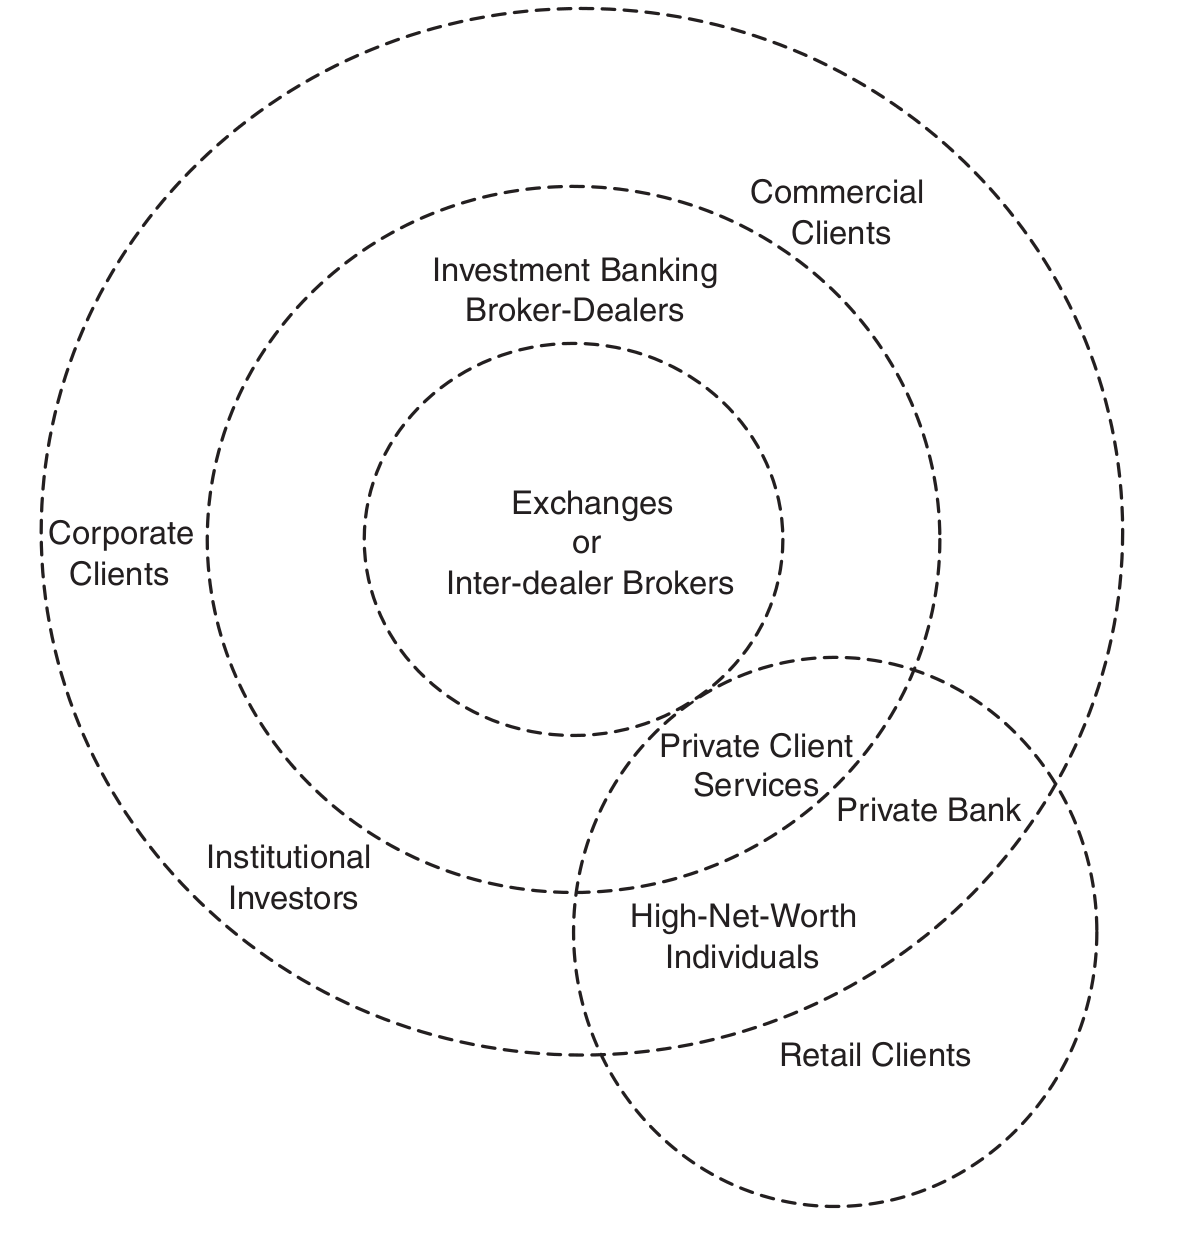
\includegraphics[width=0.7\textwidth]{img/capitalmarkets}
  \caption{Old structure of capital markets.}
  \label{fig:capitalmarket}
\end{figure}
Figure~\ref{fig:capitalmarket} shows the typical structure of capital markets
existed from the early 1929s through much of the 1990s where the broker-dealers
played the central and most profitable role.  At the core are the exchanges or
inter-dealer networks (foreign exchange trading). Exchanges are the centralized
marketplaces for transacting.  Broker-dealers perform two functions: trading for
their own accounts and transacting for their customers. Broker-dealers use
inter-dealer brokers to quickly find the best price for a particular asset among
the network of other broker-dealers. Occasionally, broker-dealers also deal
directly with other broker-dealers, particularly for less liquid instruments.
Broker-dealers clients are institutional investors, corporate clients,
commercial clients, and high-net-worth individuals.



This centralized structure existed until computer technology allowed a better
communication structure. Today financial markets are more descentralized
providing more liquidity. Exchanges and inter-dealer brokers were replaced by
liquidity pools or Electronic Communication Networks (ECNs) which are able to
transmit order quickly matching buyers and sellers optimally. There are also
dark liquidity pools where trader identity and orders remain anonymous.

Figure~\ref{fig:capitalmarketnow} shows current structucture of capital markets
including ECNs and darl pools. In this structure, ECNs, Exchanges, dark pools,
broker-dealers and retail brokerages can execute orders. However, there are some
institutional clients have also become broke-dealers.

\begin{figure}[!h]
  %\vspace{-0.8cm}
  \centering
  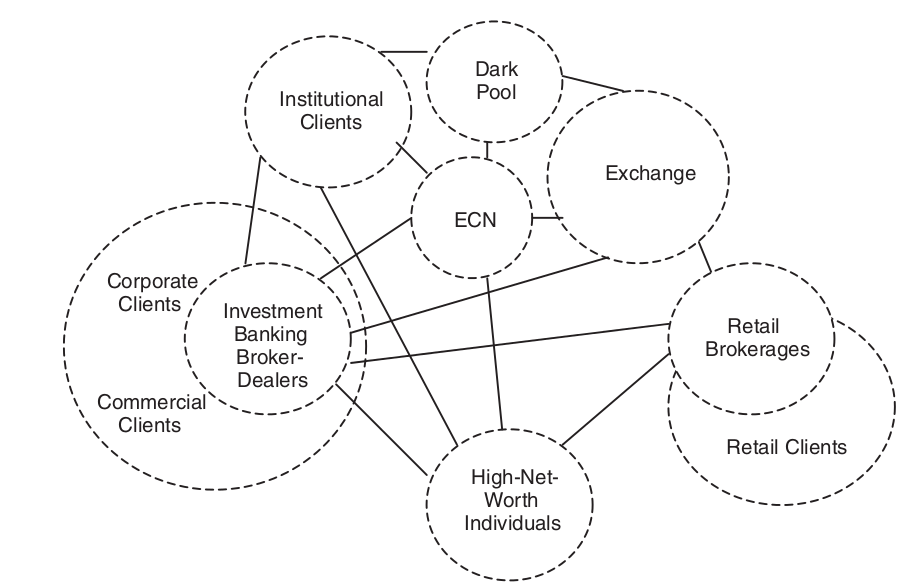
\includegraphics[width=0.8\textwidth]{img/capitalmarketsnow}
  \caption{Actual structure of capital markets.}
  \label{fig:capitalmarketnow}
\end{figure}



Equity market and foreign exchange market (Forex) are the most populat markets
for high frequency trading strategies. In equity markets can be traded stocks
such as futures and options, exchange-traded funds (ETFs) among others financial
instruments.

Forex market allows the trading of interest rates denominated pair currencies
such as EURUSD or USDJPY. Traders of this market are diverse, some of them are
high frequency traders, long-term investors and corporations. The Forex market
used to be centralized, only commercial banks had exclusive access to
inter-dealer networks. Today, Forex market is descentralized and has become the
biggest market in terms of volume of trading. The main participants are
international banks geographically dispersed with continuous 24 hours operations
excepting weekends. Figure~\ref{fig:Forextimes} shows different market trading
hours in GMT for London, New York, Sydney and Tokyo.

\begin{figure}[!h]
  %\vspace{-0.8cm}
  \centering
  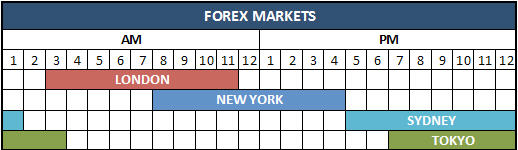
\includegraphics[width=0.8\textwidth]{img/forex-trading-hours}
  \caption{Forex market trading hours (GMT).}
  \label{fig:Forextimes}
\end{figure}

\section{Price formation process}

A trade consists at least of two orders: one to enter the market (buy order) and
exit the market (sell order). Traders have different types of order they can
execute:

\begin{description}
\item[Market order:] allow to buy or sell an asset at the current best price
whatever that price is. The transaction price is determined by the market
considering previous executed orders and volume requested.
\item[Limit order:] allow to specify the price you want to buy or sell an asset.
Depending on the market conditions, this type of orders can neven be executed.
\item[Stop order:] are suitable for investors who are unable to monitor their
investments for a period of time. Stop order allow to specify the price that a
position should be closed called stop price. When the stop price is reached a
market order is executed, this means that market price won't be exactly the same
specified in the stop order.
\end{description}

In terms of commissions, limit order are more expensive than market orders and
there is no certainty of execution.

Moreover, all orders can specify other parameters such as: 

\begin{description}
\item[Fill or Kill:] is an order that must be executed inmediately or being
cancelled, no partial fulfillments are allowed. 
\item[Day:] the order is only valid during the day.
\item[Good til canceled:] a order is active until the investor decides to cancel
ir or the trade is executed.
\end{description}

In order to determine the execution price, buyers and sellers orders are placed
in an order book which help to determine which order can be fulfilled.
Figure~\ref{fig:orderbook} illustrates how buyers and sellers are ordered. The
ask or offer price is the current lower price a seller is willing to accept for
a good. The bid price corresponds to the current highest price a buyer is
willing to pay for a good. Orders with the same price are prioritorized by
arrival time and placed on top of the book.  The difference between ask and bid
price is called spread.

\begin{figure}[!h]
  %\vspace{-0.8cm}
  \centering
  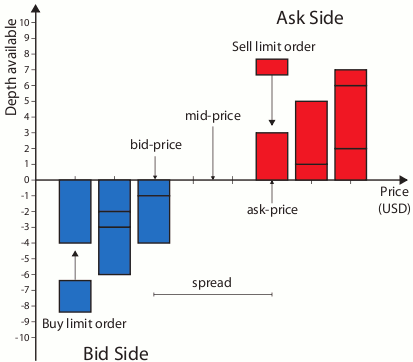
\includegraphics[width=0.5\textwidth]{img/orderbook}
  \caption{Order book. Buyers and sellers are ordered according to the bid or
  ask price and the market determines the mid-price and transacted volume.}
  \label{fig:orderbook}
\end{figure}

Today, order books are available and they are a popular source of study among
researchers. To determine the mid-price and spread modeling are some of the
problems studied.




\section{Stylized facts of asset returns}
\label{sec:stylizedfacts}

There are several known features exhibited by financial instruments called
stylized facts, which have been empirically studied and some of them have been
documented only recently and accepted as truth. Stylized facts are usually
formulated in terms of qualitative properties of asset returns and may not be
precise enought to distinguish among different parametric models.
\cite{cont2001}.

Returns of a time series $y$ is defined as:
\begin{equation}
\label{eq:returndef}
r_t = y_t - y_{t-1}  \, ,
\end{equation}

Some stylized facts which are common to a wide set of financial assets
\cite{sewell2011} are:

\begin{description}
\item[Dependence] autocorrelation in returns is largely insignificant. However,
autocorrelation in the absolute and squared returns is always positive and
significant and decays slowly. In addition, the autocorrelation in the absolute
returns is generally higher than the autocorrelation in the corresponding
squared returns.
\item[Distribution] The distribution of returns is approximately symmetric and
has high kurtosis (i.e fat tails and a peaked centre compared with the normal
distribution). However, distribution of returns whose were obtained from higher
frequencies looks more like a normal distribution.
\item[Heterogeneity] despite the fact that financial returns are non-stationary,
stationary periods can be observed. Economist speaks in terms of a structural
break \cite{stock1994}, in machine learning this is known as drift which means
that the statistical properties of the target variable change over time
\cite{widmer1996}, \cite{tsymbal2004}.
\item[Non-Linearity] financial returns may be non-linear in mean and/or
non-linear in variance.
\item[Calendar effects] are also called seasonal effects and they are cyclical
anomalies in returns where the cycle is based on the calendar. Some of known
calendar effects are: intraday effect, weekend effect, Monday effect, intramonth
effect, the January effect and Holiday effect. The most important calendar
anomalies are the January effect and the weekend effect. Figure
\ref{fig:mondayeffect} shows the Monday effect from 1928 to 2007. It shows that
in average Monday has negative returns. However, this is changing in time,
figure \ref{fig:mondayeffect2} shows returns only for year 2007 and its last
three months and it shows that Mondays and Wednesdays has positive returns in
average.

\begin{figure}[h!]
\centering
\begin{subfigure}[b]{0.45\textwidth}
 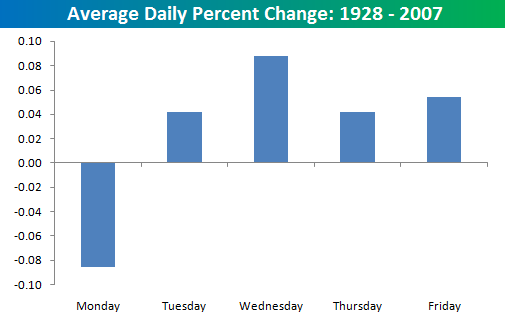
\includegraphics[width=\textwidth]{img/average_daily_change_1928_2007}
 \caption{Average daily return: 1928-2007}
 \label{fig:mondayeffect}
\end{subfigure}
\begin{subfigure}[b]{0.45\textwidth}
 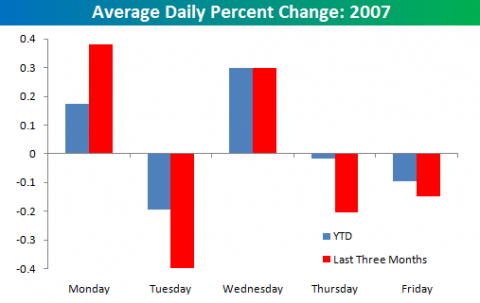
\includegraphics[width=\textwidth]{img/thumb-average_daily_change_2007}
 \caption{Average daily return: 2007}
 \label{fig:mondayeffect2}
\end{subfigure}
\end{figure}

\end{description}

\begin{description}
 \item[Dependence] 
 
 The returns
 autocorrelation function (ACF) of SPY is shown in figure
 \ref{fig:returnacf}.The figure shows how the correlations are significant even
 for very long lags, this imply that a long-memory process because of its
 long-range dependence. 
 Moreover, volatility tends to cluster, i.e. high volatility
 periods are generally followed by high volatility periods.
 
 \begin{figure}[h]
 \centering
 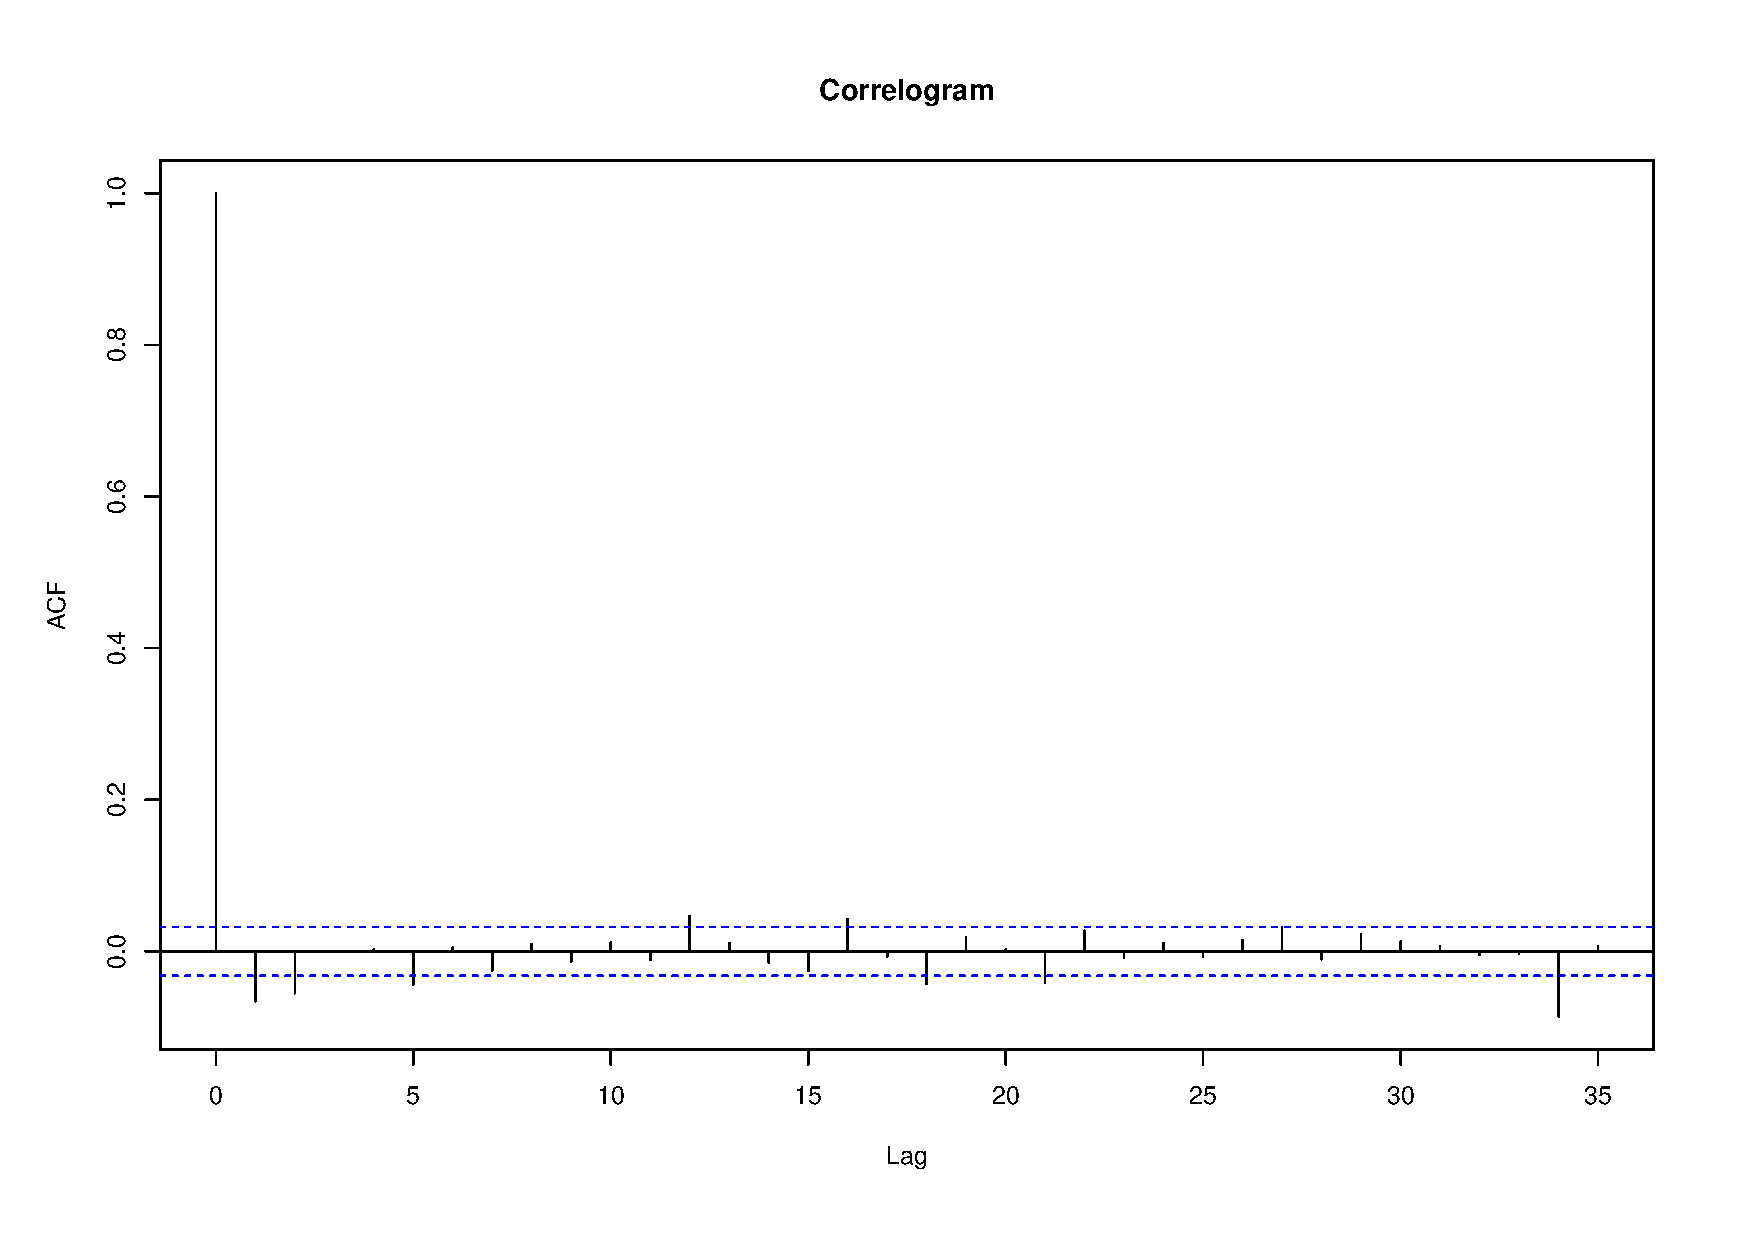
\includegraphics[width=0.9\textwidth]{plots/spy_returns_acf.pdf}
 % spy_returns_dist.pdf: 504x504 pixel, 72dpi, 17.78x17.78 cm, bb=0 0 504 504
 \caption{SPY returns ACF}
 \label{fig:returnacf}
\end{figure}


 \item[Returns distribution] The returns distribution has fat tails, i.e. the
 number of extreme events (either positive or negative) returns is larger than
 what is hypothesized by common data generation process (generally normal
 distribution assumption). In the markets, fat tails are an undesirable feature
 because of the additional risk they imply.  In the figure \ref{fig:returndist}
 is shown the SPY returns distribution based on daily dates from the period 1st
 July 1998 to 4th April 2013. The distribution was compared against the normal
 distribution which clearly doesn't fit the data.  
 \begin{figure}[h]
 \centering
 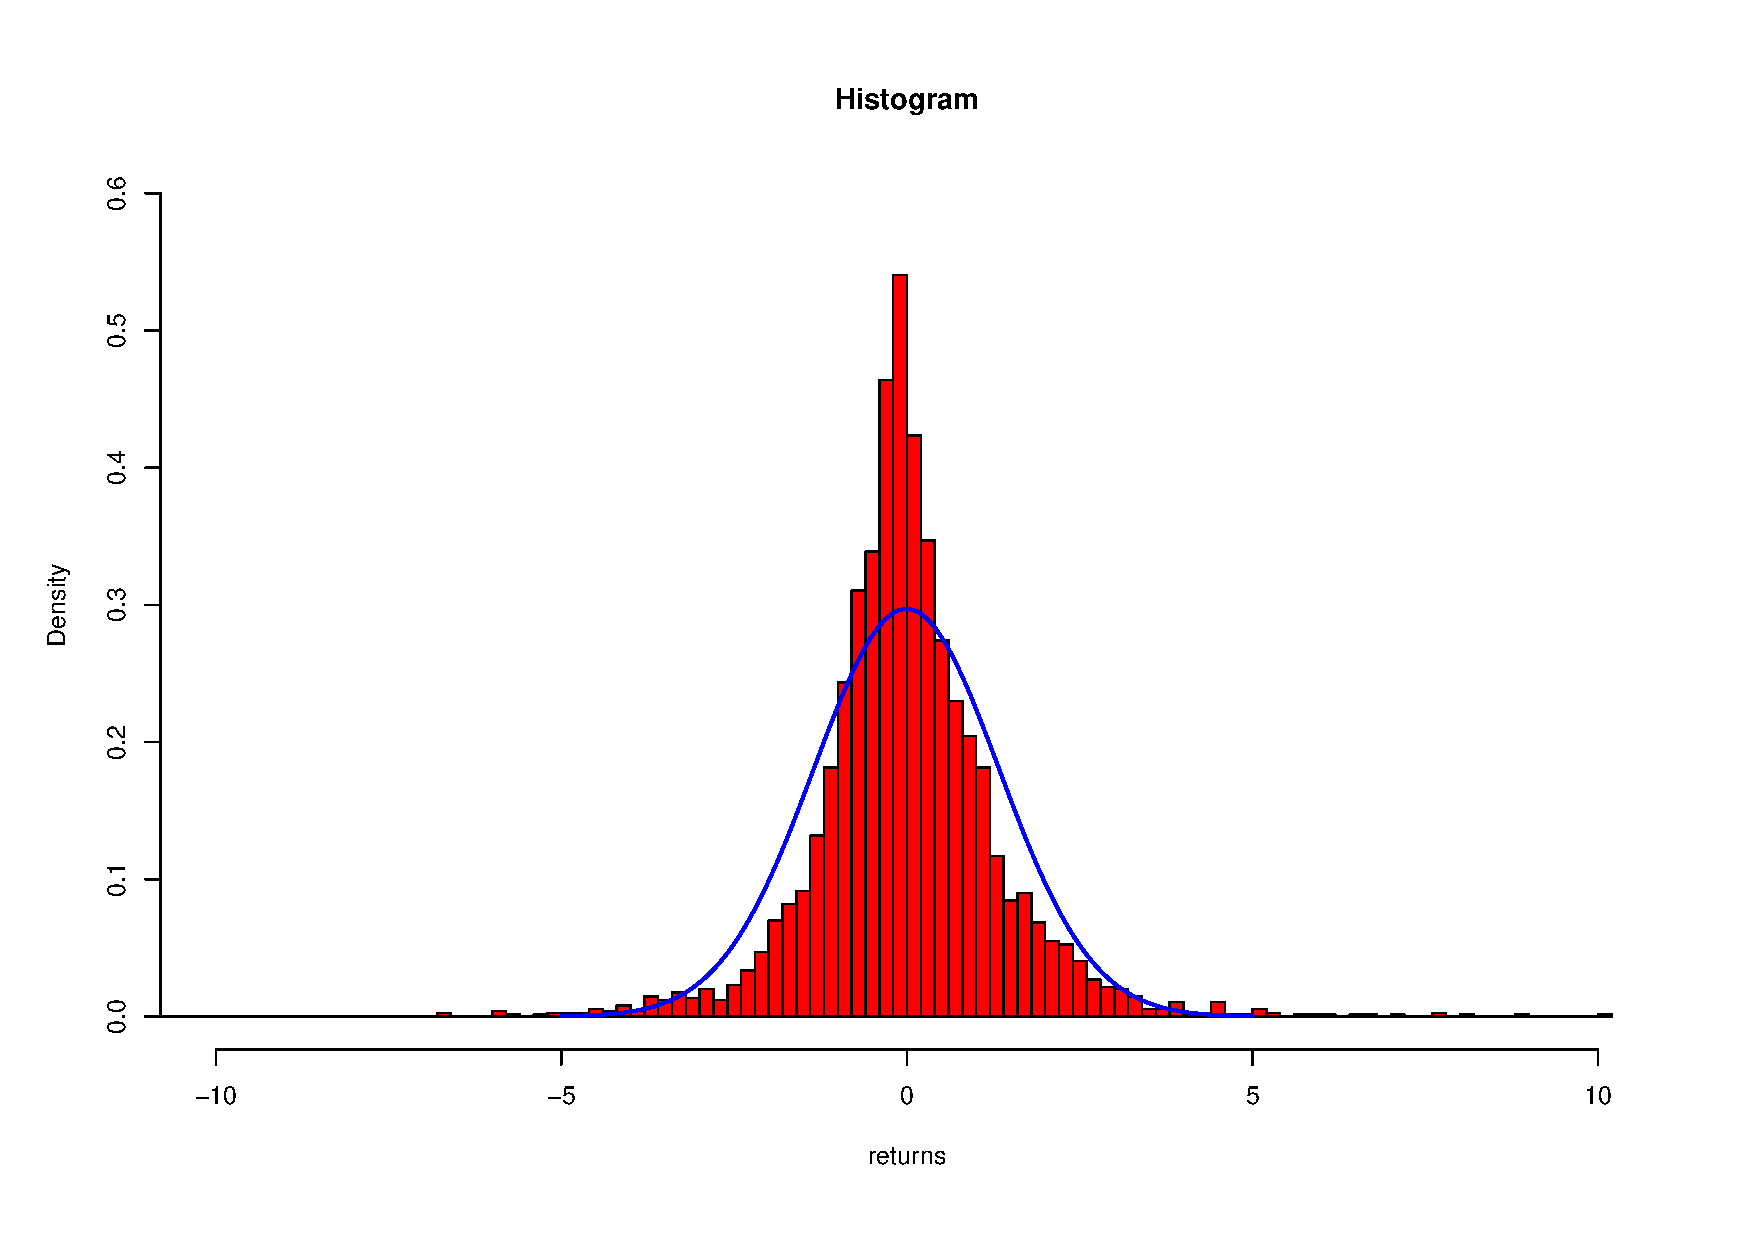
\includegraphics[scale=0.5]{plots/spy_returns_dist.pdf}
 % spy_returns_dist.pdf: 504x504 pixel, 72dpi, 17.78x17.78 cm, bb=0 0 504 504
 \caption{SPY returns distribution}
 \label{fig:returndist}
\end{figure}
 \item[Volume] refers to the level of trading activity in a market.
 \item[Calendar effects] days of week, weekend, holidays.
 \item[Intraday effects] time of the day.
 \item[Overnight effects]
\end{description}



\section{Efficient market hypothesis}

\section{Volatility in the financial markets}


In financial markets, volatility is one of the key elements to model the
stochastic dynamic behaviour of financial assets. This is mainly because
volatility gives a measure of uncertainty about future returns and it is often
viewed as an indicator of the vulnerability of financial markets. It is also
important as an input parameter in problems like derivative pricing, hedging
and portfolio management.  For example, in option pricing we need to known
first the volatility of the underlying asset before pricing an option. 

Besides, volatility provides important information for studying asset returns
because the latter are largely uncorrelated and nonlinearly dependent. However,
it has been found that volatility exhibits significant autocorrelation and
predictable patterns~\cite{poon+granger2003} and  many models have been
proposed to forecast its behaviour. 

The volatility of the data is due to a large number of factors affecting the
market, with some of them directly measurable such as historical prices,
trends, supply and demand. However, others such as monetary policies and news
are not directly measurable and are included in other models out of the scope
of this thesis. 


\subsubsection{Types of volatility}

The volatility of a stock is not directly observable~\cite{tsay2005,engle1993}. For example, daily volatility is not directly observable from only daily returns because there is only one observation in a trading day.  If intraday data is available, then volatility could be estimated. However, intraday returns are not the only explanatory variables for volatility and several estimators have been proposed. These estimators are observable variables that are related to the latent variable of interest called volatility proxies~\cite{devilderetal2007}. Examples of volatility proxies are the following: 


\begin{description}
\item[realized volatility:] is also known as historic volatility and
it is the actual variance in the price of a stock over time.
Realized volatility is measured in terms of the standard deviation
using the historical stock prices. It is commonly calculated based on
intraday price returns:
\begin{equation}
\label{eq:retintra}
r_{t,n}=100(\ln(p_{t,n}) - \ln(p_{t,n-1}))
\end{equation}
\noindent where $p_{t,n}$ is the price observed at day $t=1,\dots,T$ and
intraday sample $n=2,\dots,N$. Realized volatility is defined as:
\begin{equation}
\label{eq:rv}
    \hat{\sigma}(t) = \sum_{n=1}^N r_{t,n}^2 \, , 
\end{equation}
\noindent where $N$ is the number of intraday samples and $T$ is the
number of days. 
In order to include overnight returns, Hansen and
Lunde~\cite{hansen+lunde2005} introduced a scaling version of
realized volatility using the following definitions:
\begin{eqnarray}
r_{t}&=&100(\ln(p_{t,N}) - \ln(p_{t-1,N})) \label{eq: ret 1} \\
\bar{\rho}(t) &=& \sum_{t=1}^T r_{t}^2  \label{eq: ret 2} \, .
\end{eqnarray}
\noindent where equation~(\ref{eq: ret 1}) represents overnight 
returns and the volatility as 
equation~(\ref{eq: ret 2}), where $p_{t,N}$ is the last intraday 
sample at day $t$. The scaled realized volatility $\rho(t)$ is 
defined as:
\begin{eqnarray}
\label{eq:srv}
\rho(t) = \gamma \hat{\rho}(t) \, , \qquad & \qquad \gamma = \displaystyle \frac{\bar{\rho}(t)}{\displaystyle\sum_{t=1}^T \hat{\rho}(t)}
\end{eqnarray}
Realized volatility has also been defined as the absolute value return or as
the mean of the sum of intraday squared returns at short intervals of time. The
majority of research carried out in the literature obtain the daily volatility
as the daily squared returns as is shown in equation~(\ref{eq: ret 2}).
However, it has been proven that this measurement noise is too high for
observing the true volatility process~\cite{andersen+bollerslev1998}. Hansen
and Lunde~\cite{hansen+lunde2006} stated that the use of a noisy proxy could
result in an inferior model being chosen as the best one. The realized
volatility, as calculated by the cumulative sum of squared intraday returns and
shown in equation (\ref{eq:rv}), is less noisy and doesn't lead to choosing an
inferior model.   
\item[implied volatility:] volatility not only can be extracted from returns
but it can also be derived from option or future pricing models.  The
volatility obtained corresponds to the market's prediction of future
volatility. In finance, an option is a derivative, that is, a contract which
gives the owner the right, but not the obligation to buy or sell an underlying
asset at a given price called strike price. An option can be executed at any
time before an expiration date previously defined no matter what price the
underlying asset has. For example, the Black-Scholes model~\cite{black1973}
determines the fair option value based on stock price, strike price, time to
option expiration, the interest rate and volatility. These are known or can be
easily obtained from the market, excepting by volatility which must be
estimated. However, rather than assuming a volatility a priori and computing
option prices from it, the model can be used to estimate volatility at given
prices, time to expiration and strike price. This obtained volatility is called
the implied volatility of an option. Additionally, some models obtain implied
volatility from futures (other derivative from prices). For instance, the
Barone-Adesi and Whaley futures option model~\cite{baroneetal1987} is also used
to determine future volatilities~\cite{hamidetal2004}. Higher implied
volatility is indicative of greater price fluctuation in either direction.
Implied volatility is found by determining the value which makes theoretical
prices equal to market prices. In this way volatility is ``implied'' by the
current market price of the stock.
\end{description}


For trading strategies, the interest is centred in forecasting realized
volatility over the life of an option and to take advantage when this
volatility differs from the implied volatility. This is called volatility
arbitrage. For example, a trader will buy an option and hedge the underlying
asset if the implied volatility is under the realized volatility. 


\subsubsection{Volatility methods}

In the existing literature, there are four main classes of asset
return volatility models: the general autoregressive conditional
heteroskedasticity (GARCH) models, the stochastic volatility (SV)
models, the realized volatility models and the machine learning based
models. A comparison of the first three models can be found
in~\cite{wei2012}. 

For many years the most popular methods for estimating financial
volatility were the autoregressive conditional heteroskedasticity
(ARCH) models~\cite{engle1982} and the general ARCH (GARCH)
models~\cite{bollerslev1986}. For instance, the GARCH(1,1) defines
returns $y_t$ and volatility $\sigma_t$ as:

\begin{eqnarray*}
    y_t &=& \sigma_t \epsilon_t \\
     \sigma_t^2 &=& \alpha_0 + \alpha_1 \epsilon_{t-1}^2 + \beta_1
     \sigma_{t-1}^2
\end{eqnarray*}

\noindent where $\epsilon_t$ is standard Gaussian white noise,
$\alpha_0,\alpha_1,\beta_1 \geq 0$ are required to ensure that the
variance will never be negative and $\alpha_1+\beta_1 <1$ is needed to
guarantee a weakly stationary process~\cite{nelson1990}.

Since the introduction of the GARCH models, several extensions have been
proposed, but none of them seems to beat the GARCH(1,1)
model~\cite{lunde+hansen2005}. Despite its popularity, GARCH models have
several limitations: firstly, a time series model may be non-linear in mean
and/or non-linear in variance, but ARCH and GARCH models are non-linear in
variance, but not in mean. Besides, GARCH models often fail to capture highly
irregular phenomena, like wild market fluctuations.  

SV models explain how volatility varies in a random fashion. These models are
useful because they explain why options with different strikes and expirations
dates have different Black-Scholes implied volatilities, phenomenon known as
the volatility smile. This is useful because the Black-Scholes model assumes
that the volatility of the underlying asset is constant which is not always
true. There are several SV models and the most well-known and popular is the
Heston model~\cite{heston1993}. Additional information about SV models can be
found in~\cite{shephard1995}. 

The realized volatility constructed from high frequency intraday returns gave
rise to the realized volatility models mainly because the realized volatility
series is much more homoskedastic and seems to be a long memory
process~\cite{andersonetal2003}. For realized volatility, the autoregressive
fractionally integrated moving average (ARFIMA) process emerged as a standard
model~\cite{chenetal2010} and many variations have been studied, but all of
them produce similar forecasting results to the ARFIMA(1,d,1)
model~\cite{koopmanetal2005}.  

On the other hand, machine learning based models, especially artificial neural
networks (ANN) and support vector machines (SVM) have arisen as an alternative
to forecast volatility. ANN is a statistical technique inspired by biological
neural networks which is capable of changing its structure based on external or
internal information during a training phase~\cite{sammut2011}. SVM are
supervised learning models for classification analysis which recognize patterns
finding a separating hyperplane. An extension for regression analysis is known
as support vector regression (SVR). 

Since machine learning models and in particular ANN do not require assumptions
about the data (gaussianity for example) and allow more explanatory variables
than returns to be included, they have become widely used in solving financial
problems, specially volatility
forecasting~\cite{hamidetal2004,donaldsonetal1997}. There are also many works
focused on the using of SVM in volatility
forecasting~\cite{shiyietal2008,shiyietal2010,gavrishchaka2006,vasilios2012}. 

However, just as with ANN, SVMs have scalability problems because their
training process is computationally intensive and it is done in batch mode. The
scalability problem worsens when new additional training data is available and
a re-training process from scratch needs to be done. This problem can be
avoided using online machine learning algorithms that allow one instance at a
time to be processed with low computationally expensive calculations.




%Volatility models have been extensively
%studied~\cite{gatheral2006,poon+granger2003,knight2002} and some of  them
%include machine learning
%methods~\cite{hamidetal2004,donaldsonetal1997,shiyietal2008,shiyietal2010,gavrishchaka2006,vasilios2012}.  
%
